%----------------------------------------------------------------------------------------
%	PACKAGES AND OTHER DOCUMENT CONFIGURATIONS
%----------------------------------------------------------------------------------------

\documentclass[12pt, a4paper]{report}
\usepackage[english]{babel}
\usepackage[utf8x]{inputenc}
\usepackage{amsmath}
\usepackage{graphicx}
\usepackage[colorinlistoftodos]{todonotes}
\usepackage{fancyhdr}
\usepackage{float}
\usepackage{lastpage}
\usepackage{ tipa }
\usepackage{graphicx, wrapfig, subcaption, booktabs}
\usepackage{makecell}
\usepackage[T1]{fontenc}
\usepackage{fourier}
\usepackage{multirow}
\usepackage[protrusion=true, expansion=true]{microtype}
\usepackage{url, lipsum}
\usepackage[nottoc]{tocbibind}
\usepackage{siunitx}
\usepackage{listings}
\usepackage{ amssymb }
\usepackage{hyperref}
\usepackage{ upgreek }
\usepackage{ stmaryrd }

\usepackage{geometry}
\geometry{
 a4paper,
 total={210mm,297mm},
 left=40mm,
 top=30mm,
 bottom=20mm,
 right=20mm, 
}

\renewcommand{\bibsection}{}

\usepackage{amsthm}
\theoremstyle{definition}
\newtheorem{definition}{Definition}
\usepackage{sectsty}
\allsectionsfont{\centering \normalfont\scshape}

\numberwithin{equation}{chapter}		
\numberwithin{figure}{chapter}		
\numberwithin{table}{chapter}	

%\sectionfont{\Large}

\usepackage{titlesec}
%\titleformat{\chapter}{\bfseries\huge}{\thechapter.}{20pt}{\huge}
\titleformat{\chapter}[display] { \centering \normalfont\Large \bfseries \scshape}{\chaptertitlename\ \thechapter}{0pt}{\Large}
\titlespacing{\chapter}{1cm}{1cm}{1cm}


\chapternumberfont{\Large \centering \scshape} 
\chaptertitlefont{\Large \centering \scshape}

\DeclareMathOperator*{\argmin}{arg\,min}


\usepackage{setspace}
\doublespacing

%Roman Numbers Snippet
\makeatletter
\newcommand{\rmnum}[1]{\romannumeral #1}
\newcommand{\Rmnum}[1]{\expandafter\@slowromancap\romannumeral #1@}
\makeatother

\begin{document}

\pagenumbering{roman}

\begin{spacing}{1.5}
\begin{titlepage}

%\newcommand{\HRule}{\rule{\linewidth}{0.5mm}} % Defines a new command for the horizontal lines, change thickness here

\center % Center everything on the page
 
%----------------------------------------------------------------------------------------
%	TITLE SECTION
%----------------------------------------------------------------------------------------


\includegraphics{./Pics/unsw_logo.png} \\ [0.5cm]

{ \textsc{\LARGE Mycroft - An AI approach to detect }} \\ [0.5cm]
{ \textsc{\LARGE Semantic Data Types using NLP }} \\ [0.5cm]
{ \textsc{\LARGE and Deep Learning}}\\[1.5cm]

{ \large Shashank Reddy Boosi} \\[2.0cm]
{\large A thesis in fulfilment of the requirements for the degree} \\ [0.25cm]
{\large of Master of Information Technology}\\[1.5cm]


{\textsc{\large School of Computer Science and Engineering}}\\[1.0cm]

{ \large August 25, 2020}\\[1.5cm]

{\large Supervisor: Dr. Wei Wang}

\end{titlepage}
\end{spacing}

\begin{spacing}{1.5}
\chapter*{ORIGINALITY STATEMENT}
\setlength{\parskip}{2.2em}
\setlength{\parindent}{0em}
I hereby declare that this submission is my own work and to the best of my knowledge
it contains no materials previously published or written by another person,
or substantial proportions of material which have been accepted for the award of
any other degree or diploma at UNSW or any other educational institution, except
where due acknowledgement is made in the thesis. Any contribution made to the
research by others, with whom I have worked at UNSW or elsewhere, is explicitly
acknowledged in the thesis. I also declare that the intellectual content of this thesis
is the product of my own work, except to the extent that assistance from others in
the projects design and conception or in style, presentation and linguistic expression
is acknowledged.

\end{spacing}

%\vspace*{0.2cm}
\begin{spacing}{1.5}
\chapter*{ACKNOWLEDGEMENT}
\setlength{\parskip}{2.2em}
\setlength{\parindent}{0em}
I would like to express my profound gratitude to my advisor, \textbf{Dr.Wei Wang, Professor} for his support and encouragement of my research project, for sharing his immense knowledge. His guidance helped me to face new challenges that were involved in tackling the project.
\par 
\setlength{\parskip}{2.2em}
\setlength{\parindent}{0em}
Besides the advisor, I would like to thank  \textbf{Yifang Sun, Research Associate} for his guidance which helped me through difficult situations. I am grateful for all the insights he had which helped me navigate and understand the project better. 
\par 
\setlength{\parskip}{2.2em}
\setlength{\parindent}{0em}
My sincere thanks to \textbf{Yukai Miao} who helped me to get the access and also set up the environment in a CSE lab machine. He was pretty prompt which helped me to set up very quickly.
\par 
\setlength{\parskip}{2.2em}
\setlength{\parindent}{0em}
I deeply thank my family and friends for supporting me in all the tasks that I have carried for the successful completion of this project.
\end{spacing}

\begin{spacing}{1.5}
\vspace*{0.5cm}
\tableofcontents
\end{spacing}

\begin{minipage}{\textwidth}
\begin{spacing}{1.5}
\vspace*{0.5cm}
\listoffigures
\listoftables
\newpage
\end{spacing}
\end{minipage}

\begin{spacing}{2}
\chapter*{ABBREVIATIONS}
\setlength{\parskip}{2.2em}
\setlength{\parindent}{0em}
\textbf{AI} \hspace*{1.35cm} Artificial Intelligence \\
\textbf{CRF} \hspace*{1cm} Conditional Random Field \\
\textbf{DL} \hspace*{1.2cm} Deep Learning \\
\textbf{LSTM} \hspace*{0.8cm} Long Short-Term Memory \\
\textbf{NLP} \hspace*{1cm} Natural Language Processing \\
\textbf{NN} \hspace*{1.2cm} Neural Network \\
\textbf{STD} \hspace*{1cm} Standard Deviation \\
\textbf{WDC} \hspace*{0.85cm} Web Data Commons \\ 

\end{spacing}
\newpage

\begin{spacing}{1.5}
\chapter*{ABSTRACT}
\setlength{\parskip}{2.2em}
\setlength{\parindent}{0em}
Detecting data types has been achieved using traditional methods of computer science but semantic data type detection is a challenge because it involves a lot of parameters to consider, especially with the number of semantic types being different for every environment and semantic data types are essential for data mining tasks like data discovery, schema detection, schema matching, and data cleaning, etc. Present day methods to detect semantic types are not robust as their accuracy of detecting is very low. The dataset that we use is taken from WDC 2015 \cite{wdc} where we train on a different range of web tables ranging from 40000 to 100000 and extract the data columns which range from 10529 to 26143 by matching 78 semantic types from DBpedia to column headers \cite{dbpedia}. We map each data column that is being produced from the Web tables into 1588 features using different NLP feature characteristics and then train the features on the model that is being tuned for the dataset. We achieved a accuracy, weighted F1-score, precision and recall of 49.464, 49.870, 54.025 and 49.464 respectively for the dataset produced using 100000 web tables.
\par 
\setlength{\parskip}{2.2em}
\setlength{\parindent}{0em}
\textsc{\textbf{KEYWORDS}}: Semantic Type Detection, NLP, Web Tables, Deep Learning, LSTM.

\end{spacing}
%%---------------------------------Introduction ----------------------------------------------

\pagenumbering{arabic}


\chapter{INTRODUCTION}
\begin{spacing}{1.5}
\setlength{\parindent}{0em}
Many Data Mining tasks like data preparation, analysis, discovery rely on the detecting types to infer rules and constraints on the functionality of the process. Automatic detection of these types is very important which facilitates validation, transformation rules, data statistics, similarities across columns all which are dependant on these types. While many systems still depend on the pre-existing types like string, boolean etc., Semantic types will give us the leverage to perform more cases. Knowing about a value type is very essential in a lot of applications and types like location, birth date, name have quite a different structure in different places and there is a lot of ambiguity in the dataset because of that. Many commercial tool analytics like Microsoft Power BI \cite{powerbi} and Tableau \cite{tableau} are currently relying on the standard methods like ontology based methods, regular expression patterns, dictionary lookups of the column headers to detect the semantic types but the number of types are limited and are pertained to the non ambiguous ones. Our goal is to improve the performance of these semantic types irrespective of their value structure.
\par
\setlength{\parskip}{2.2em}
\setlength{\parindent}{0em}
In this project, we considered WDC 2015 Web table corpus \cite{wdc} as our dataset where we extracted the data from the tables with only 78 semantic types which are described in the T2Dv2 Gold Standard \cite{t2dv2}, which matches properties from DBpedia \cite{dbpedia, wttodbpedia} with column headers from the corpus. Then we do the exact match between the semantic types that we considered and column headers in the web tables which are extracted in relation with the table orientation. Our transformation after this will consists of a mapping between the column headers with their respective values. We then extract 1,588 features from each column by combining the likes of character level distribution, baseline statistics, word embeddings and paragraph vectors. We then train these features on a novel sequence supported neural network model which achieves a weighted F1-score of 49.870, competing with that of the other baseline models in the same dataset proportion.

\chapter{RELATED WORKS}
\label{chap:rw}
\setlength{\parindent}{0em}
Semantic Type Detection has a lot of important applications in many tasks like commercial data preparation, discovery and this kind of detection will help us define, match schemas and will make the life of many data science and AI tasks easier and our work is mainly inspired from Sherlock  \cite{sherlock} where they strive to solve this problem using Neural networks like the way we do and we compare our model with Sherlock model as we consider Sherlock to be the standard for Semantic Type detection using DL. 
\par
\setlength{\parskip}{2.2em}
\setlength{\parindent}{0em}
Many commercial tool these days are relying on ontology based methods, regular expression patterns, dictionary lookups of the column headers to detect the semantic types but the types are limited.  Open source libraries like messytables \cite{messytables}, datalib \cite{datalib} use these kinds of heuristics and detect the limited types but remain infeasible due to the amount of semantic types that are available in the data mining tasks. 
\par
\setlength{\parskip}{2.2em}
\setlength{\parindent}{0em}
Due to the high uncertainty of the values of the semantic types, many methods like ontology based, feature based and probabilistic based algorithms couldn't succeed in producing a standard algorithm that will get us close to solving the detection. In ontology based, many researchers tried to use the data from Web Tables \cite{webtable}, DBpedia \cite{dbpedia, wttodbpedia}, Wikitology \cite{30} to convert these tables into key-value mappings and use the maximum likelihood estimators where Wikitology \cite{30} helps with the idea of using the column headers and their values to form the dataset.
\par
\setlength{\parskip}{2.2em}
\setlength{\parindent}{0em}
In feature based, where the data is converted into features which is ontology agnostic. Ramnandan et al. \cite{27} use Term Frequency and Inverse Document Frequency (TF-IDF)  by first separating the numerical and textual types whereas Pham et al. \cite{23} uses slightly more features and their approach is mainly based on extracting similarities of the textual data to train the ML models. Sherlock leverages this kinds of approaches and uses a significantly large varieties of feature characteristics which includes character distributions, word embeddings and paragraph vectors to train the Neural network models.
\par
\setlength{\parskip}{2.2em}
\setlength{\parindent}{0em}
Finally, in probabilistic based approaches, they use inference procedure by considering a few inferences to detect the semantic types. Goel et al. \cite{11} uses CRF to predict the semantic types based on the values in a column and also assuming that every column is related to the other column in terms of frequency occurrence with in a web table. Limaye et al. \cite{19} uses probabilistic models to consider value as entities, columns as entity types and column pairs with relationships for the graphical model and our approach is quite similar to the probabilistic based models.
\end{spacing}


\chapter{METHODOLOGY}
\begin{spacing}{1.5}
The methodology explains the process flow as shown in the figure \ref{fig:arcdiadram}.

\begin{figure}[h]
    \centering
    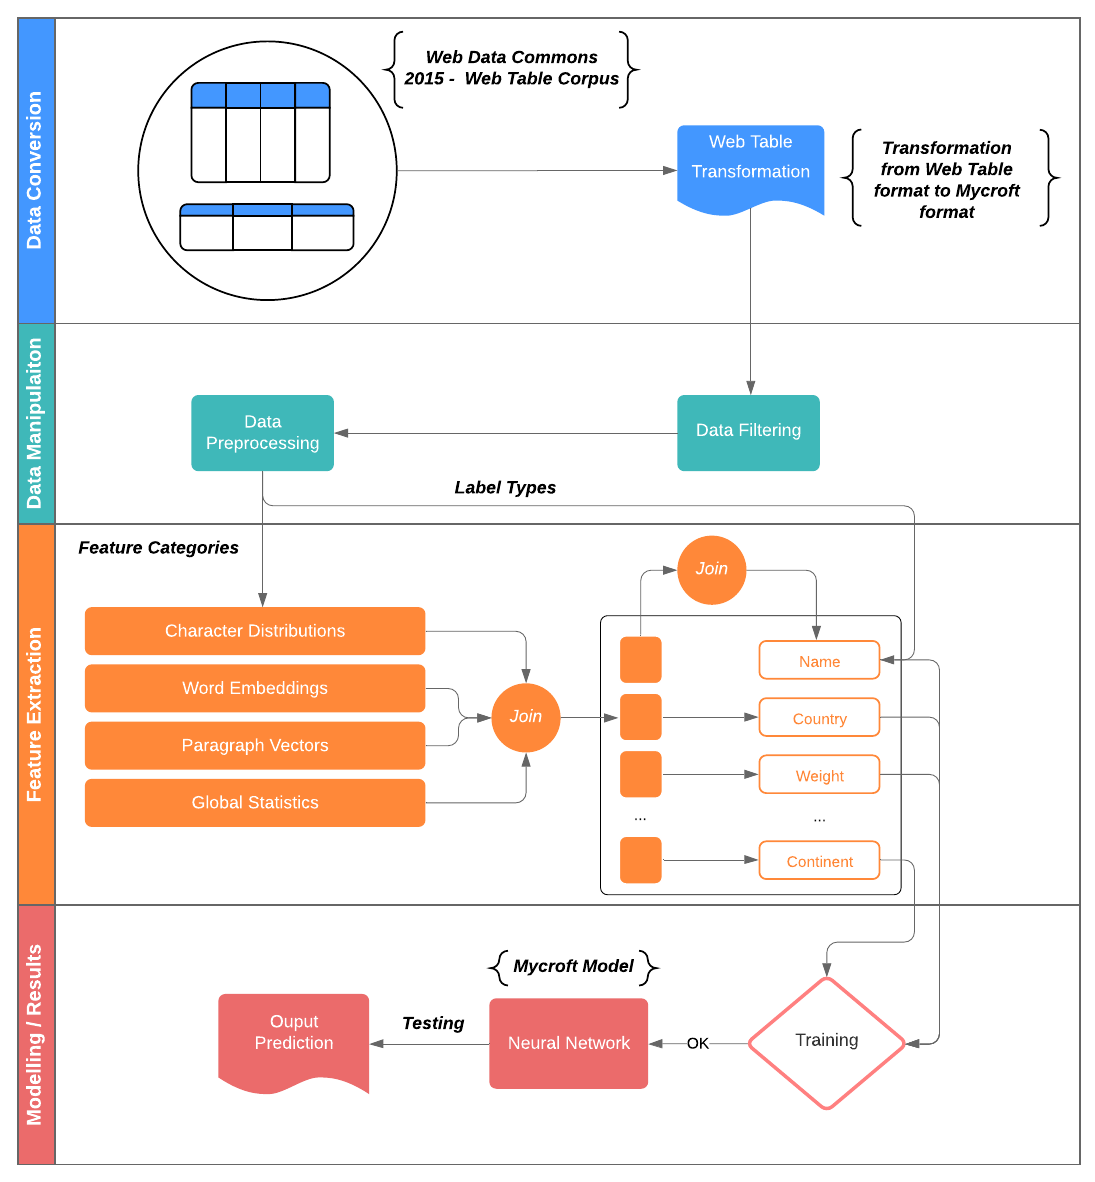
\includegraphics[width=\textwidth]{./Pics/architectural_diagram.png} 
    \caption{Mycroft Architectural Diagram}
    \label{fig:arcdiadram}
\end{figure}

\section{Data}
\label{sec:data}

In this section, we will describe how we extracted data columns from WDC Web Corpus 2015 \cite{wdc} of real-world datasets and also how we did the preprocessing and filtering of the data before extracting features.

\subsection{Data Collection}
\label{ssec:datacol}

The dataset that we choose for this project is the WDC Web Table Corpus 2015, which parsed 1.78 billion HTML pages and after filtering and preprocessing all the innermost tables which constituted to 10.24 billion, 233 million tables remain. These tables are classified into 4 categories Relational, Entity, Matrix and Layout \cite{wdc}. We only chose the Relational tables which consisted of 51 million tables.

\subsection{Data Transformation}
\label{ssec:datatra}

Every table from \ref{ssec:datacol} is represented in the form of a JSON, and every json file consisted of the attributes \textbf{relation, pageTitle, title, url, hasHeader, headerPosition, tableType, tableNum, s3Link, recordEndOffset, recordOffset, tableOrientation, TableContextTimeStampBeforeTable, TableContextTimeStampAfterTable, lastModified, hasKeyColumn, keyColumnIndex, headerRowIndex, textBeforeTable} of which most of the information is redundant for our project. So for the transformation, we mainly used the \textbf{relation} attribute which consisted of all the information we need for the project and the \textbf{tableOrientation}. We only considered the horizontal and vertical orientations and shuffled through the 78 semantic types that is being extracted from T2Dv2 Gold Standard \cite{t2dv2} and matching the types from DBpedia \cite{dbpedia} to column headers. Finally we do all this operation on 40000, 50000, 100000 web tables and extract the semantic types and their values dataset from the Web Table corpus. After transformation, the number of tuples in the dataset at this stage are 14652, 18257, 36391 for 40000, 50000 and 100000 web tables respectively.

\subsection{Data Filtering and Processing}
\label{ssec:datafil}

Once the data is transformed, we will now move forward and apply the following filtering and preprocessing techniques, so that the model can weigh in all the semantic types rather than only a few of them. They are:

\begin{itemize}
\item Remove special characters from the data.
\item Remove the data which contains more than 5 percent of the labels in the transformed data \ref{ssec:datatra}. 
\item Remove the data which contains less than 10 percent of the labels in the refined data which was extracted in the option before.
\end{itemize}

\par
\setlength{\parskip}{2.2em}
\setlength{\parindent}{0em}
Figure \ref{fig:columns} shows the number of columns extracted and their count after the data stage. After all the filtering and preprocessing the data is now ready to move on to the feature extraction stage and the number of tuples in the dataset are 10529, 13034, 26143 for 40000, 50000 and 100000 web tables respectively.


\begin{figure}[H]
    \centering
    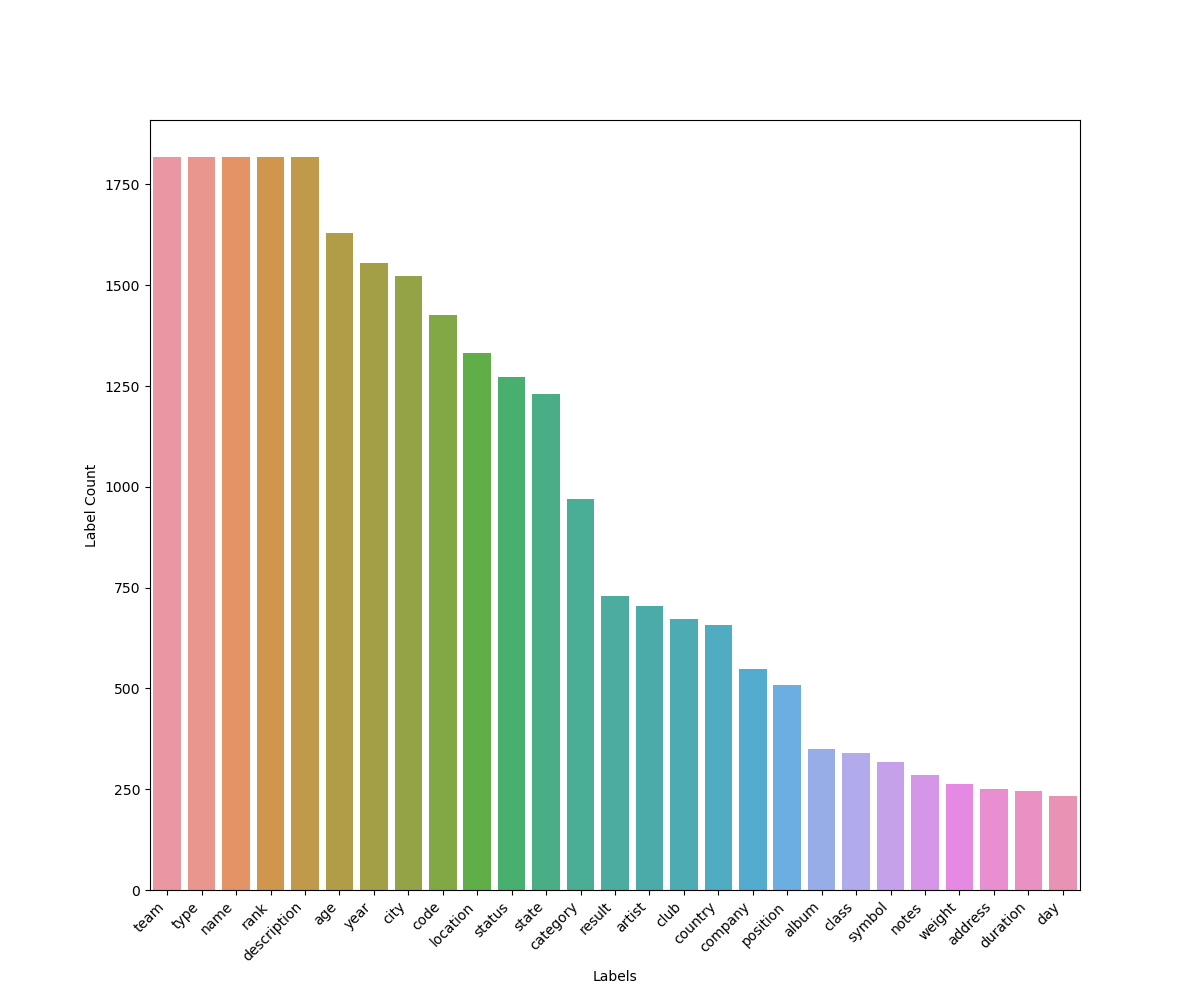
\includegraphics[width=\textwidth, height=11cm]{./Pics/label_count_100000.png} 
    \caption{Number of columns extracted from WDC and its count}
    \label{fig:columns}
\end{figure}

\section{Feature Extraction}
\label{sec:feature}

Due to the high variable change in the length of the columns in the dataset, we decided to convert into a fixed-length representation, so that the model training and result extraction would be smooth. The different kinds of feature characteristics \cite{sherlock} that are used in order to make it possible are : global statistics (27), character distributions (960), glove word embeddings (200), and self-trained paragraph vectors (400).

\subsection{Global Statistics}
\label{ssec:stat}

In this category of features, we have extracted all the high level statistical features that many researchers use to extract meaningful information out of a dataset. Information which describe how uniform the data is distributed, all the numerical features are captured by mean, std etc., All the 27 statistical features are described in the table \ref{table:1}

\begin{table}[H]
\begin{tabular}{l} 
\hline
\textbf{Feature Description} \\
\hline
Number of values. \\ 
Column entropy. \\ 
Fraction of values with unique content. \\ 
Fraction of values with numerical characters. \\ 
Fraction of values with alphabetical characters. \\ 
Mean and std. of the number of numerical characters in values. \\ 
Mean and std. of the number of alphabetical characters in values. \\ 
Mean and std. of the number special characters in values. \\ 
Mean and std. of the number of words in values. \\ 
{Percentage, count, only/has-Boolean} of the None values. \\ 
{Stats, sum, min, max, median, mode, kurtosis, skewness,any/all-Boolean} of length of values. \\ 
\hline
\end{tabular}
\caption{Description of the 27 statistical features}
\label{table:1}
\end{table}


\subsection{Character Level Distribution}
\label{ssec:char}

Character level based matching has been quite prevalent in many researched which will give a predictive power to the output and as shown in Sherlock \cite{sherlock} it contributes a lot towards the end results. 
In the character level distributions, we will convert every character in the column and distribute across the 96 ASCII-printable characters which include digits, letters, punctuations ,special characters except the white space. Once the mapping is done, we aggregate all these character counts with 10 statistical features namely any, all, mean, variance, min, max, median, sum, kurtosis, skewness resulting in 960 features.

\subsection{Word Embeddings}
\label{ssec:word}

Word embeddings are one of the most popular text based feature extraction technique used in many data science and AI tasks where we use high dimensional fixed-length vectors to represent words. In this project, we used a pre-trained Glove dictionary \cite{glove} containing 50 dimensional representation which consists of 400K English words. For each value in a column, we lookup the value in the Glove dictionary, and omit if the term does not exist and multiple words are looked up separately and we take the mean of the vectors as a whole. Finally, once the lookup and mapping is done we calculate the mean, mode, median and variance of the word vectors across all the values in a column adding up 201 dimensions into out feature vector.

\subsection{Paragraph Vectors}
\label{ssec:para}

Finally the last technique that we used to convert text into fixed-length numerical vectors is by using Distributed Bag of Words version of Paragraph vector \cite{para}. We will assume every column to be a \textbf{paragraph} and each and every value in a column to be \textbf{words} and the whole structure is represented by one-hot encoded vectors.
\par
\setlength{\parskip}{2.2em}
\setlength{\parindent}{0em}
After we pool all columns together across the classes, we will randomly select a window of value vectors and train the model to predict the former from latter by using gensim library \cite{gensim} over every 20 iterations. Once training is done we will map the columns to a 400 dimensional paragraph vector which will provide us with better predictive power over both training and test sets.


\section{Neural Network: Mycroft Model}
\label{sec:nn}

The models used to train and test Semantic type detection are very simple models like traditional statistical models, Machine Learning models such as Logistic Regression, Regular Expression etc., but their functionality is only restricted to a small feature set and these algorithms couldn't account for the high variability of the values of the semantic types. Sherlock was the first of a kind model which uses multi input neural network with feed forward layers which could achieve remarkable results in the space of Semantic Type Detection. Our model is inspired from Sherlock where it could account for high variability of the values for the semantic types and also could predict many semantic types at once. The hyper parameters for the Mycroft model are shown in the table \ref{table:2}.

\begin{table}[H]
\centering
\begin{tabular}{|c| c|} 
\hline
\textbf{Hyper parameters} & \textbf{Values} \\
\hline
Metric & Accuracy, F1-score, Precision, Recall\\ 
Loss Function & Categorical Cross-Entropy\\ 
Optimizer & Adam\\ 
Epochs & 20\\ 
Early Stopping Patience & 5\\ 
Learning Rate & 1e-4\\ 
Weight Decay Rate & 1e-4\\ 
\hline
\end{tabular}
\caption{Hyperparameters used for training}
\label{table:2}
\end{table}

\setlength{\parindent}{0em}
As shown in the figure \ref{fig:nnmodel}, Mycroft NN model consists of multi inputs and each input is assigned a subnetwork and the number of inputs is based on the number of feature categories that are used in the project. We evaluate all the sub-networks individually especially 3 of the 4 subnetworks are assigned the same layers except the sub-network with the feature category of Statistical features which is just normalized and all the outputs of the sub-networks are concatenated to form the input of the primary network.
\par
\setlength{\parskip}{2.2em}
\setlength{\parindent}{0em}
Each sub-network consists of 2 Dense hidden layers with varying hidden size ranging from 100 to 400 depending on the size of the input and Relu activation function is used to scale the data and we use dropout and batch normalization to avoid overfitting of the data.
\par
\setlength{\parskip}{2.2em}
\setlength{\parindent}{0em}
The primary network consists of 3 Dense hidden layers with varying hidden sizes from 78 to 1000 and 1 bi-directional LSTM \cite{lstm} which will help us remember the sequences of the values in the columns thus boosting the performance of the model. Other than that the primary network consists of Relu activation function, dropout and batch normalization for every hidden layer. The final output results corresponds to the weights assigned to semantic type belonging to each class, the predicted label is then the class with the highest confidence. \textbf{Mycroft} model is implemented in Pytorch \cite{torch}.

\begin{figure}[h]
    \centering
    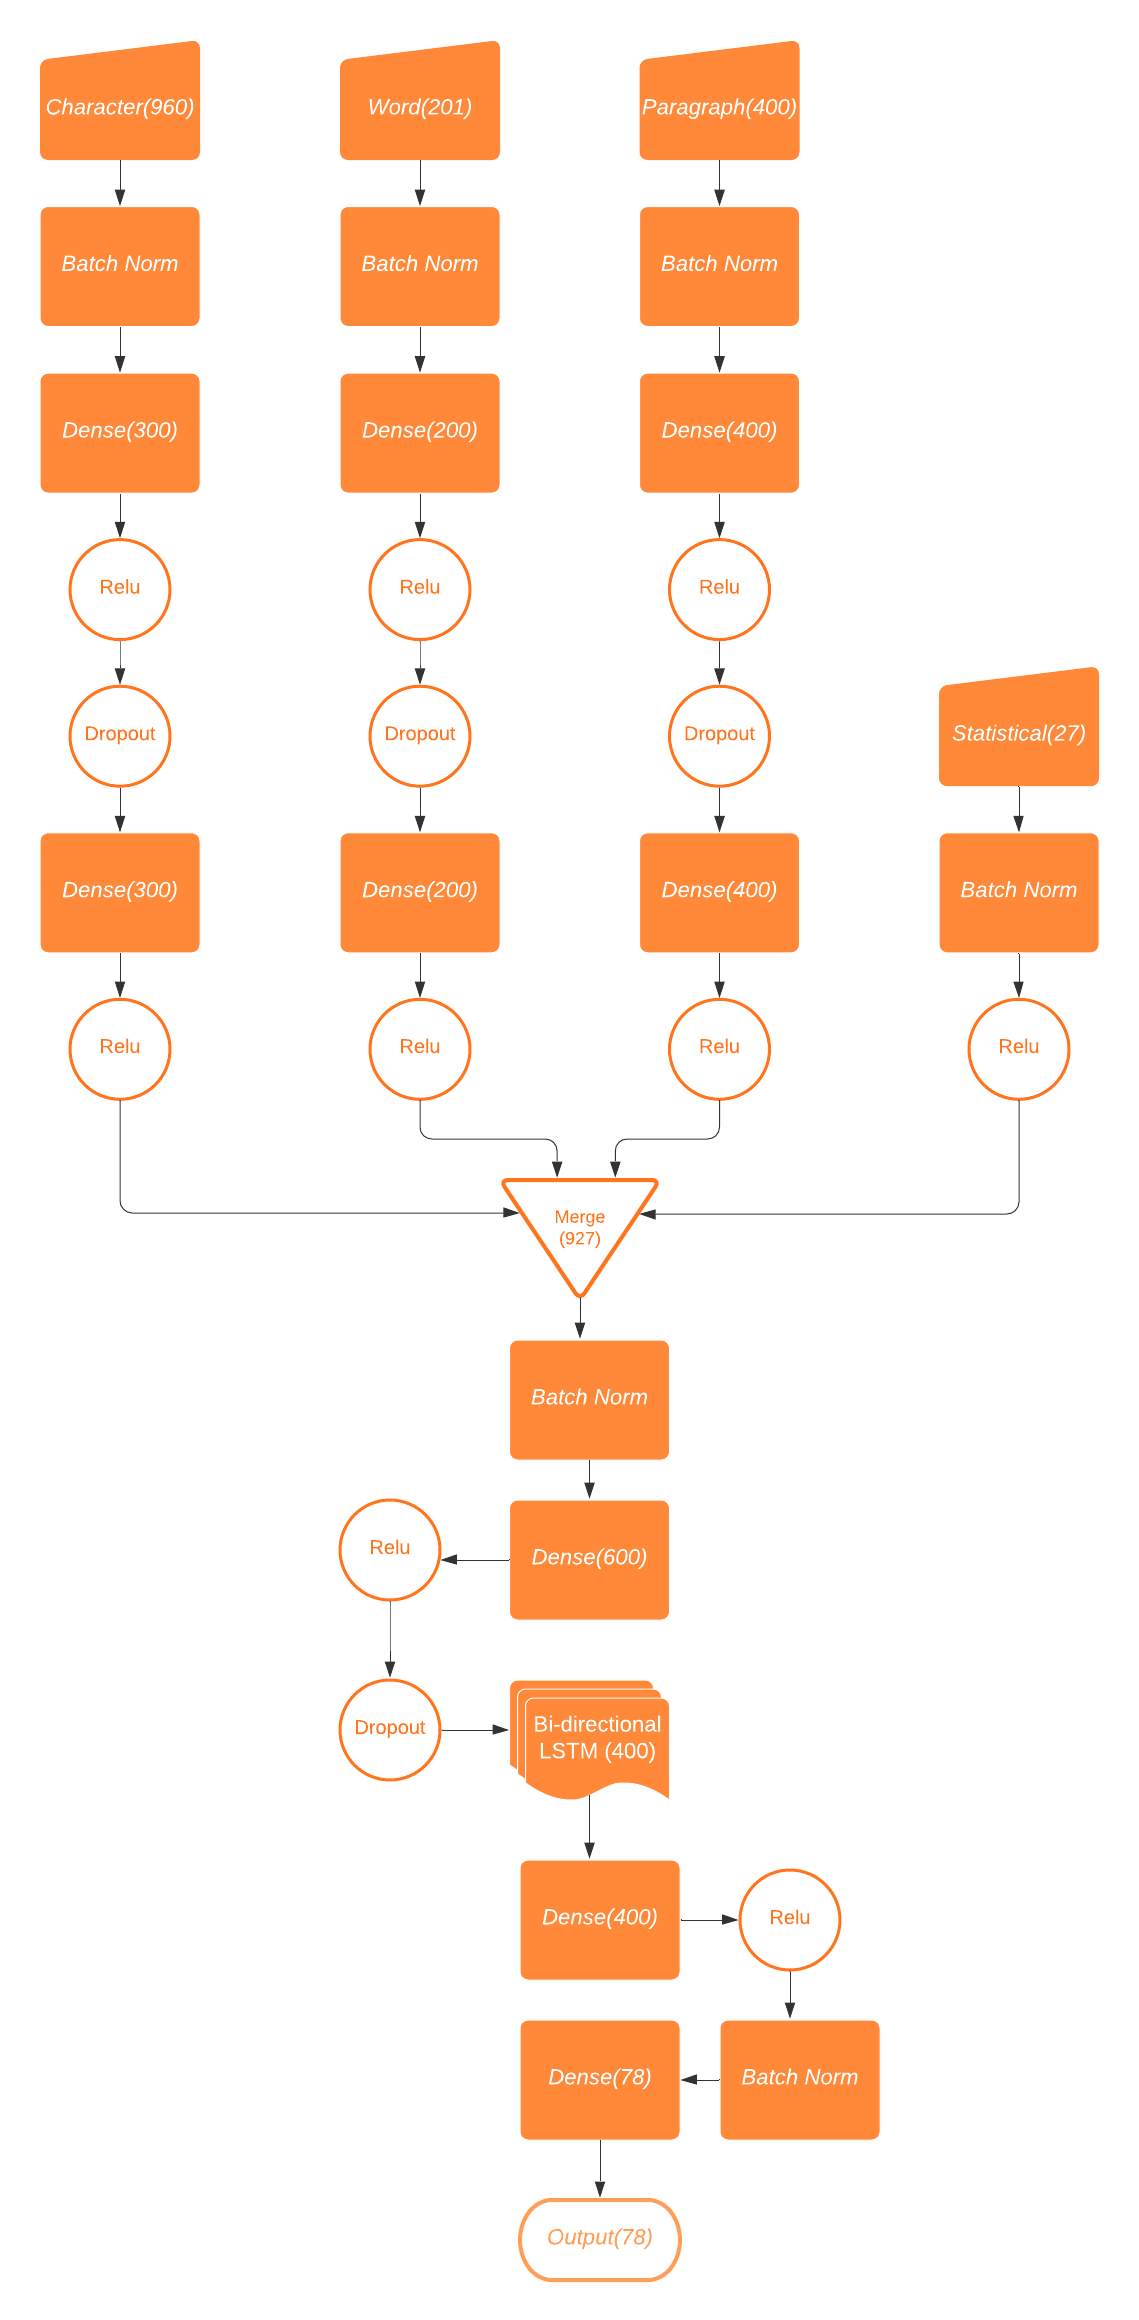
\includegraphics[height=21cm]{./Pics/nnmodel1.png} 
    \caption{Mycroft Neural Network Model}
    \label{fig:nnmodel}
\end{figure}

\subsection*{Training and Evaluation}

The dataset is divided into 80/10/10 training/validation/testing splits and to account for the class imbalances, we evaluate the model performance using weighted F1-score which is the harmonic mean of precision and recall as shown in the equation below.

\begin{equation}
F1-score = 2 × \frac{precision × recall}{precision + recall}
\end{equation}

We will also calculate categorical accuracy, recall, precision. The average time taken was in the feature extraction process which took 8 seconds per column.

\end{spacing}


\chapter{RESULTS AND ANALYSIS}
\begin{spacing}{1.5}

\section*{Experiments}

Many different kinds of experiments are performed to achieve the optimal hyper parameters that are suitable for our dataset. Table \ref{table:3} shows the the comparison between Sherlock \cite{sherlock} and Mycroft with the sample data. The reason for comparing the 2 models using the sample data is because this sample is the only dataset that is provided by Sherlock with its results. And after running our model against the same data, we outperformed Sherlock both in terms of accuracy and F1-score and the margin of success is too high because of the use of sequence based algorithm LSTM which gives us the extra predictive power by handling the high variability of the values in the dataset.
\par
\setlength{\parskip}{1em}

\begin{table}[H]
\centering
\begin{tabular}{| c | c | c | } 
\hline
& \textbf{Sherlock} & \textbf{Mycroft} \\ [0.5ex]
\hline
Accuracy in \% & 82.52 & 95.20\\ 
F1-score in \% & 82.72 & 94.88\\ 
\hline
\end{tabular}
\caption{Accuracy and F1-score comparison between Sherlock \cite{sherlock} and Mycroft on the sample}
\label{table:3}
\end{table}

\par
\setlength{\parindent}{0em}
\setlength{\parskip}{1em}
Once the comparison with the samples is completed we wanted to explore this model by experimenting on the WDC Web Table Corpus 2015 by choosing 3 different datasets of 40000, 50000 and 100000 web tables respectively. Table \ref{table:4} shows the metrics accuracy, F1-score, precision and recall for all the 3 different web table sizes. As you can see in the table, the bigger the size of the web tables gets, the greater the predictive power of the overall model. We experimented this results by only choosing 1 percent of the size of what Sherlock used in order to get their results and yet our results are on par and challenging with Sherlock evaluations. The main focus was calculating the weighted F1-score which takes into account the variability of each classes by weighing them accordingly.
\par
\setlength{\parskip}{1em}

\begin{table}[H]
\centering
\begin{tabular}{ | c | c | c | c | c | } 
\hline
Web Tables & \textbf{Accuracy in \%} & \textbf{F1-score in \%} & \textbf{Precision in \%} & \textbf{Recall in \%} \\ [0.5ex]
\hline
40000& 44.919 & 44.225 & 46.353 & 44.919 \\ 
50000& 45.168 & 45.127 & 47.826 & 45.168 \\ 
100000& 49.464 & 49.870 & 54.025 & 49.464 \\
\hline
\end{tabular}
\caption{Accuracy, F1-score, precision, recall for different size of web tables \cite{wdc}}
\label{table:4}
\end{table}

\par
\setlength{\parindent}{0em}
\setlength{\parskip}{1em}
As seen in the figure \ref{fig:accweb}, which is a graph between the number of epochs versus the accuracy for different web tables, the accuracy with the 100000 web tables is high right from the beginning when compared to the other web table size. This is because of the dataset being trained with more data which in turn reduces the variability of semantic type values. We can also see that the lines are not in a smooth incremental curve and this is also due to the high uncertainty of the values being exposed while training. 

\begin{figure}[h]
    \centering
    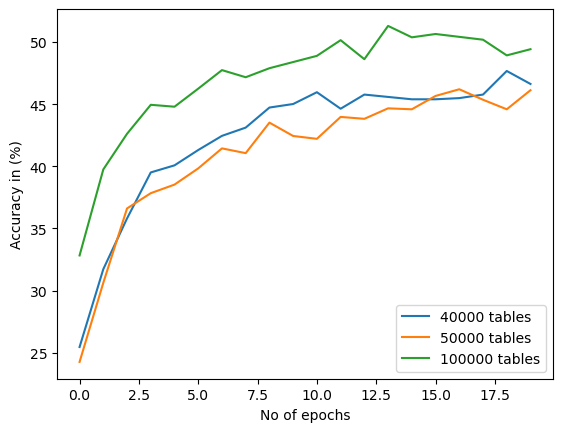
\includegraphics[width=\textwidth]{./Pics/accuracy.png} 
    \caption{Number of epochs vs validation accuracy graph between different web tables}
    \label{fig:accweb}
\end{figure}

\end{spacing}

\chapter{CONCLUSION AND FUTURE WORKS}
\begin{spacing}{1.5}
\setlength{\parindent}{0em}
In conclusion, detecting semantic types is very important in solving many important data science and AI related tasks and we have explored a way to improve the process of detecting the semantic types and the results of this outcome looked more promising as we used sequence based algorithms in our model which gave the boost in performance in terms of all metrics used.
\par
\setlength{\parindent}{0em}
\setlength{\parskip}{2.2em}
We can further develop the process by applying Conditional Random Fields \cite{crf} like linear chain and ordering based etc., to leverage the similarity in terms of the Web Table structure. We can also reduce the uncertainty in the dataset by using more web tables as used in Sherlock \cite{sherlock}, which will help us gather different values in the semantic types thus avoiding outlier values whilst testing.

\end{spacing}
\newpage

%%------------------------------------------End Conclusion--------------------------------

%%----------------------------------Start bibtex -----------------------------------------
\bibliographystyle{ieeetr}
\renewcommand{\bibname}{References}
\bibliography{references}

%-----------------------------------End bibtex--------------------------------------------

\end{document}
